\documentclass[12pt]{report}

% Packages
\usepackage{acronym}
\usepackage{amsmath}
\usepackage{amsthm}
\usepackage{amsfonts}
\usepackage{epigraph}
\usepackage{geometry}
\usepackage{graphicx}
%\usepackage{mdframed}
\usepackage{titlesec}
\usepackage{caption}
\usepackage{listings}
\usepackage{xcolor}
\usepackage{siunitx}
\usepackage{enumitem}
\usepackage{pdfpages}
\usepackage[utf8]{inputenc}
\usepackage{fancyhdr}
\usepackage{transparent}
\usepackage[hidelinks, colorlinks=true, linkcolor=blue, urlcolor=blue, citecolor=blue]{hyperref}
\usepackage[backend=biber, style=ieee]{biblatex}
%\addbibresource{cdt_app.bib}

% Acronym set-up
% Command to insert acronyms with a temporary color change
\newcommand{\myAcro}[1]{{\hypersetup{linkcolor=black}\acl{#1}}} % For acronym list (full form)
\newcommand{\myAcroLink}[1]{{\hypersetup{linkcolor=black}\acs{#1}}}

% Document geometry setup
\geometry{
    a4paper,
    margin=2cm,
    top=1cm,    % Adjust top margin
    bottom=1cm,  % Adjust bottom margin
    headheight=14.5pt,
    includeheadfoot
}

\pagestyle{fancy} % Use fancy style for all pages
\fancyhf{} % Clear all header and footer fields

% Header
\fancyhead[L]{{\transparent{0.5}Chapter \udlchap{} Questions}} % Left header
\fancyhead[R]{{\transparent{0.5}wp289}} % Right header

% Footer
\fancyfoot[L]{\transparent{0.5}Understanding Deep Learning} % Left footer
\fancyfoot[R]{\transparent{0.5}\thepage} % Right footer

% Define line thickness
\renewcommand{\headrulewidth}{0.4pt}
\renewcommand{\footrulewidth}{0.4pt}

% Redefining plain page style if needed
\fancypagestyle{plain}{ % Applies to chapter beginnings and similar
  \fancyhf{} % clear all header and footer fields for plain style
  \renewcommand{\headrulewidth}{0.4pt}
  \renewcommand{\footrulewidth}{0.4pt}
  \fancyhead[L]{{\transparent{0.5}Chapter \udlchap{}Questions}}
  \fancyhead[R]{{\transparent{0.5}wp289}}
  \fancyfoot[L]{\transparent{0.5}Understanding Deep Learning}
  \fancyfoot[R]{\transparent{0.5}\thepage}
}

% Customise Chapter Headings
\titleformat{\chapter}
    {\normalfont\LARGE\bfseries}
    {\thechapter.}
    {1em}
    {}
\titlespacing*{\chapter}{0pt}{-20pt}{\baselineskip}

% Customise section spacing
\titlespacing*{\section}{0pt}{\baselineskip}{0.5\baselineskip}

% Adjusting space around figures
\setlength{\floatsep}{5pt}
\setlength{\textfloatsep}{5pt}

% Adjusting caption spacing
\captionsetup{aboveskip=5pt, belowskip=5pt}

% Format paragraphs
\setlength{\parindent}{0pt}
\setlength{\parskip}{1em}  % Adjust the value as needed

% Adjust list spacing
%\setlist[enumerate]{before=\vspace{0.5em}, after=\vspace{0.5em}}
\setlist[enumerate]{before=\vspace{-0.5\baselineskip}, after=\vspace{-0.5\baselineskip}}

% Customise question boxes
\usepackage[framemethod=TikZ]{mdframed}
\mdfsetup{
    backgroundcolor=gray!20,
    innertopmargin=10pt,
    innerbottommargin=10pt,
    skipbelow=0pt 
}

\def\udlchap{11}
\renewcommand{\thesubsection}{Problem \udlchap.\arabic{subsection}}

%%%%%%%%%%%%%%%%%%%%%%%%%%%%%%%%%%%%%%%%%%%%%%%%%%%%%%%%%

\begin{document}

\section*{Chapter 11: Residual Networks}

\subsection{}
\begin{mdframed}
    Derive equation 11.5 from the network definition in equation 11.4.

    \begin{align*}
        \mathbf{h}_{1} & = \mathbf{x} + \mathbf{f}_{1}[\mathbf{x}, \boldsymbol{\phi}_{1}]         \\
        \mathbf{h}_{2} & = \mathbf{h}_{1} + \mathbf{f}_{2}[\mathbf{h}_{1}, \boldsymbol{\phi}_{2}] \\
        \mathbf{h}_{3} & = \mathbf{h}_{2} + \mathbf{f}_{3}[\mathbf{h}_{2}, \boldsymbol{\phi}_{3}] \\
        \mathbf{y}     & = \mathbf{h}_{3} + \mathbf{f}_{4}[\mathbf{h}_{3}, \boldsymbol{\phi}_{4}]
        \label{eq:11.4}
        \tag{11.4}
    \end{align*}

    \begin{align*}
        \mathbf{y} & = \mathbf{x} + \mathbf{f}_{1}[\mathbf{x}]                                                                                                                                                                                               \\
                   & + \mathbf{f}_{2}[\mathbf{x} + \mathbf{f}_{1}[\mathbf{x}]]                                                                                                                                                                               \\
                   & + \mathbf{f}_{3}[\mathbf{x} + \mathbf{f}_{1}[\mathbf{x}] + \mathbf{f}_{2}[\mathbf{x} + \mathbf{f}_{1}[\mathbf{x}]]]                                                                                                                     \\
                   & + \mathbf{f}_{4}[\mathbf{x} + \mathbf{f}_{1}[\mathbf{x}] + \mathbf{f}_{2}[\mathbf{x} + \mathbf{f}_{1}[\mathbf{x}]] + \mathbf{f}_{3}[\mathbf{x} + \mathbf{f}_{1}[\mathbf{x}] + \mathbf{f}_{2}[\mathbf{x} + \mathbf{f}_{1}[\mathbf{x}]]]]
        \label{eq:11.5}
        \tag{11.5}
    \end{align*}
\end{mdframed}

Substituting $\mathbf{h}_{3}$ into $\mathbf{y}$, we get:

\begin{equation}
    \mathbf{y} = \mathbf{h}_{2} + \mathbf{f}_{3}[\mathbf{h}_{2}, \boldsymbol{\phi}_{3}] + \mathbf{f}_{4}[\mathbf{h}_{2} + \mathbf{f}_{3}[\mathbf{h}_{2}, \boldsymbol{\phi}_{3}], \boldsymbol{\phi}_{4}]
    \label{eq:h3_y}
\end{equation}

Next, substitute $\mathbf{h}_{2}$ into Equation~\eqref{eq:h3_y}:

\begin{equation}
    \mathbf{y} = \mathbf{h}_{1} + \mathbf{f}_{2}[\mathbf{h}_{1}, \boldsymbol{\phi}_{2}] + \mathbf{f}_{3}[\mathbf{h}_{1} + \mathbf{f}_{2}[\mathbf{h}_{1}, \boldsymbol{\phi}_{2}], \boldsymbol{\phi}_{3}] + \mathbf{f}_{4}[\mathbf{h}_{1} + \mathbf{f}_{2}[\mathbf{h}_{1}, \boldsymbol{\phi}_{2}] + \mathbf{f}_{3}[\mathbf{h}_{1} + \mathbf{f}_{2}[\mathbf{h}_{1}, \boldsymbol{\phi}_{2}], \boldsymbol{\phi}_{3}], \boldsymbol{\phi}_{4}]
\end{equation}

Finally, substitute $\mathbf{h}_{1}$ into the above equation:

\begin{align*}
    \mathbf{y} & = \mathbf{x} + \mathbf{f}_{1}[\mathbf{x}, \boldsymbol{\phi}_{1}]                                                                                                                                                                                                                                                                                                                                                                        \\
               & + \mathbf{f}_{2}[\mathbf{x} + \mathbf{f}_{1}[\mathbf{x}, \boldsymbol{\phi}_{1}], \boldsymbol{\phi}_{2}]                                                                                                                                                                                                                                                                                                                                 \\
               & + \mathbf{f}_{3}[\mathbf{x} + \mathbf{f}_{1}[\mathbf{x}, \boldsymbol{\phi}_{1}] + \mathbf{f}_{2}[\mathbf{x} + \mathbf{f}_{1}[\mathbf{x}, \boldsymbol{\phi}_{1}], \boldsymbol{\phi}_{2}], \boldsymbol{\phi}_{3}]                                                                                                                                                                                                                         \\
               & + \mathbf{f}_{4}[\mathbf{x} + \mathbf{f}_{1}[\mathbf{x}, \boldsymbol{\phi}_{1}] + \mathbf{f}_{2}[\mathbf{x} + \mathbf{f}_{1}[\mathbf{x}, \boldsymbol{\phi}_{1}], \boldsymbol{\phi}_{2}] + \mathbf{f}_{3}[\mathbf{x} + \mathbf{f}_{1}[\mathbf{x}, \boldsymbol{\phi}_{1}] + \mathbf{f}_{2}[\mathbf{x} + \mathbf{f}_{1}[\mathbf{x}, \boldsymbol{\phi}_{1}], \boldsymbol{\phi}_{2}], \boldsymbol{\phi}_{3}], \boldsymbol{\phi}_{4}] \tag{3}
    \label{eq:11.3}
\end{align*}

Equation~\eqref{eq:11.3} is equivalent (without the $\phi$ parameters shown) to Equation~\eqref{eq:11.5} as required.

\newpage

\subsection{}
\begin{mdframed}
    Unraveling the four-block network in figure 1a produces one path of length zero, four paths of length one, six paths of length two, four paths of length three, and one path of length four. How many paths of each length would there be if with (i) three residual blocks and (ii) five residual blocks? Deduce the rule for $K$ residual blocks
\end{mdframed}

\begin{figure}[ht]
    \centering
    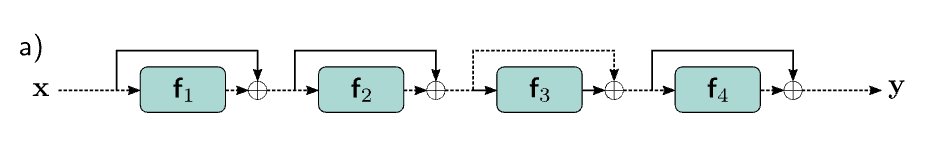
\includegraphics[width=\textwidth]{11_4.png}
    \caption{Four-block network}
    \label{fig:11.4a}
\end{figure}

The path of length zero stems from the input $\mathbf{x}$ directly connecting to output $\mathbf{y}$ without passing through any residual blocks. The number of paths of length zero is always one.

In summary, for a network with 4 residual blocks, the number of paths of each length is as follows:

\begin{itemize}
    \item Paths of length zero: 1
    \item Paths of length one: 4
    \item Paths of length two: 6
    \item Paths of length three: 4
    \item Paths of length four: 1
    \item Total paths: 16
\end{itemize}

For a network with 3 residual blocks, the number of paths of each length is as follows:

\begin{itemize}
    \item Paths of length zero: 1
    \item Paths of length one: 3
    \item Paths of length two: 3
    \item Paths of length three: 1
    \item Total paths: 8
\end{itemize}

For a network with 5 residual blocks, the number of paths of each length is as follows:

\begin{itemize}
    \item Paths of length zero: 1
    \item Paths of length one: 5
    \item Paths of length two: 10
    \item Paths of length three: 10
    \item Paths of length four: 5
    \item Paths of length five: 1
    \item Total paths: 32
\end{itemize}

For $K$ residual blocks, the number of paths for each length is given by $\binom{K}{l}$ where $K$ is the number of residual blocks, and $l$ is the length of the path.

\begin{equation*}
    \binom{K}{l} = \frac{K!}{l!(K-l)!}
\end{equation*}

\subsection{}
\begin{mdframed}
    Show that the derivative of the network in equation 11.5 with respect to the first layer $\mathbf{f}_{1}[\mathbf{x}]$ is given by equation 11.6.

    \begin{equation}
        \frac{\partial \mathbf{y}}{\partial \mathbf{f}_{1}} = \mathbf{I} + \frac{\partial \mathbf{f}_{2}}{\partial \mathbf{f}_{1}} + \left(\frac{\partial \mathbf{f}_{3}}{\partial \mathbf{f}_{1}} + \frac{\partial \mathbf{f}_{3}}{\partial \mathbf{f}_{2}}\frac{\partial \mathbf{f}_{2}}{\partial \mathbf{f}_{1}}\right) + \left(\frac{\partial \mathbf{f}_{4}}{\partial \mathbf{f}_{1}} + \frac{\partial \mathbf{f}_{4}}{\partial \mathbf{f}_{2}}\frac{\partial \mathbf{f}_{2}}{\partial \mathbf{f}_{1}} + \frac{\partial \mathbf{f}_{4}}{\partial \mathbf{f}_{3}}\frac{\partial \mathbf{f}_{3}}{\partial \mathbf{f}_{1}} +\frac{\partial \mathbf{f}_{4}}{\partial \mathbf{f}_{3}}\frac{\partial \mathbf{f}_{3}}{\partial \mathbf{f}_{2}}\frac{\partial \mathbf{f}_{2}}{\partial \mathbf{f}_{1}}\right)
        \label{eq:11.6}
        \tag{11.6}
    \end{equation}
\end{mdframed}


\begin{align*}
    \mathbf{y} & = \mathbf{x} + \mathbf{f}_{1}[\mathbf{x}]                                                                                                                                                                                               \\
               & + \mathbf{f}_{2}[\mathbf{x} + \mathbf{f}_{1}[\mathbf{x}]]                                                                                                                                                                               \\
               & + \mathbf{f}_{3}[\mathbf{x} + \mathbf{f}_{1}[\mathbf{x}] + \mathbf{f}_{2}[\mathbf{x} + \mathbf{f}_{1}[\mathbf{x}]]]                                                                                                                     \\
               & + \mathbf{f}_{4}[\mathbf{x} + \mathbf{f}_{1}[\mathbf{x}] + \mathbf{f}_{2}[\mathbf{x} + \mathbf{f}_{1}[\mathbf{x}]] + \mathbf{f}_{3}[\mathbf{x} + \mathbf{f}_{1}[\mathbf{x}] + \mathbf{f}_{2}[\mathbf{x} + \mathbf{f}_{1}[\mathbf{x}]]]]
    \label{eq:11.5}
    \tag{11.5}
\end{align*}

First layer contribution:

\begin{equation*}
    \frac{\partial \mathbf{y}}{\partial \mathbf{f}_{1}} = \mathbf{I},
\end{equation*}

because the direct contribution of $\mathbf{f}_{1}$ to $\mathbf{y}$ is linear and independent. The second layer contribution is given by:

\begin{equation*}
    \frac{\partial \mathbf{y}}{\partial \mathbf{f}_{1}} \; \text{from} \; \mathbf{f}_{2} = \frac{\partial \mathbf{f}_{2}}{\partial (\mathbf{x}+\mathbf{f}_{1})} \cdot \frac{\partial (\mathbf{x}+\mathbf{f}_{1})}{\partial \mathbf{f}_{1}}=\frac{\partial \mathbf{f}_{2}}{\partial \mathbf{f}_{1}}
\end{equation*}

\null
Rewriting the third layer as:

\begin{equation*}
    \mathbf{z}_{3} = \mathbf{x} + \mathbf{f}_{1}[\mathbf{x}] + \mathbf{f}_{2}[\mathbf{z}_{2}]
\end{equation*}

Therefore, the direct dependency of $\mathbf{f}_{3}$ on $\mathbf{f}_{1}$ is given by:

\begin{equation*}
    \frac{\partial \mathbf{f}_{3}}{\partial \mathbf{z}_{3}} \cdot \frac{\partial \mathbf{z}_{3}}{\partial \mathbf{f}_{1}} = \frac{\partial \mathbf{f}_{3}}{\partial \mathbf{f}_{1}}
\end{equation*}

The indirect dependency of $\mathbf{f}_{3}$ on $\mathbf{f}_{1}$ is given by:

\begin{equation*}
    \frac{\partial \mathbf{f}_{3}}{\partial \mathbf{z}_{3}} \cdot \frac{\partial \mathbf{z}_{3}}{\partial \mathbf{f}_{2}} \cdot \frac{\partial \mathbf{f}_{2}}{\partial \mathbf{f}_{1}} = \frac{\partial \mathbf{f}_{3}}{\partial \mathbf{f}_{2}} \cdot \frac{\partial \mathbf{f}_{2}}{\partial \mathbf{f}_{1}}
\end{equation*}

Adding these two terms together gives the third layer contribution to the derivative of $\mathbf{y}$ with respect to $\mathbf{f}_{1}$:

\begin{equation*}
    \frac{\partial \mathbf{f}_{3}}{\partial \mathbf{f}_{1}} + \frac{\partial \mathbf{f}_{3}}{\partial \mathbf{f}_{2}} \cdot \frac{\partial \mathbf{f}_{2}}{\partial \mathbf{f}_{1}}
\end{equation*}

A similar method can be followed for the fourth layer to get the derivative of $\mathbf{y}$ with respect to $\mathbf{f}_{1}$ as given in Equation~\eqref{eq:11.6}.



\subsection{}
\begin{mdframed}
    Explain why the values in the two branches of the residual blocks in figure 11.6a are uncorrelated. Show that the variance of the sum of uncorrelated variables is the sum of their individual variances.
\end{mdframed}

The values in the two branches of the residual blocks in figure 11.6a are uncorrelated beacause the input to the main branches of the residual block is multiplied by the weight matrix, which is normally distributed with mean zero ($\Omega \sim \mathcal{N}(0, \Sigma)$). This can equally multiply by a positive or negative number, so they are uncorrelated.


The definition of variance is given by:

\begin{equation*}
    \text{Var}(X) = \mathbb{E}[X^{2}] - \mathbb{E}[X]^{2}
\end{equation*}

For two uncorrelated variables $X$ and $Y$, we want to show that the variance of their sum is the sum of their individual variances:

\begin{align*}
    \text{Var}(X + Y) & = \mathbb{E}[(X + Y)^{2}] - \mathbb{E}[(X + Y)]^{2}                                                                             \\
                      & = \mathbb{E}[X^{2} + 2XY + Y^{2}] - (\mathbb{E}[X] + \mathbb{E}[Y])^{2}                                                         \\
                      & = \mathbb{E}[X^{2}] + 2\mathbb{E}[XY] + \mathbb{E}[Y^{2}] - (\mathbb{E}[X] + \mathbb{E}[Y])^{2}                                 \\
                      & = \mathbb{E}[X^{2}] - \mathbb{E}[X]^{2} + 2\mathbb{E}[XY] - 2\mathbb{E}[X]\mathbb{E}[Y] + \mathbb{E}[Y^{2}] - \mathbb{E}[Y]^{2} \\
                      & = \mathbb{E}[X^{2}] - \mathbb{E}[X]^{2} + \mathbb{E}[Y^{2}] - \mathbb{E}[Y]^{2}                                                 \\
                      & = \text{Var}(X) + \text{Var}(Y)
\end{align*}

Where we used the fact that $X$ and $Y$ are uncorrelated so have zero covariance to go from line 4 to line 5:

\begin{equation*}
    \text{Cov}(X, Y) = \mathbb{E}[XY] - \mathbb{E}[X]\mathbb{E}[Y] = 0 \implies \mathbb{E}[XY] = \mathbb{E}[X]\mathbb{E}[Y]
\end{equation*}

\subsection{}
\begin{mdframed}
    The forward pass for batch normalisation given a batch of scalar values $\{z_{i}\}^{I}_{i=1}$ consists of the following operations:

    \begin{alignat*}{2}
        f_{1}  & = \mathbb{E}[z_{i}]  & \quad f_{5}  & = \sqrt{f_{4}+\epsilon}         \\
        f_{2i} & = x_{i} - f_{1}      & \quad f_{6}  & = \frac{1}{f_{5}}               \\
        f_{3i} & = f_{2i}^{2}         & \quad f_{7i} & = f_{2i} \times f_{6}           \\
        f_{4}  & = \mathbb{E}[f_{3i}] & \quad z'_{i} & = f_{7i} \times \gamma + \delta \\
        \label{eq:11.10}
        \tag{11.10}
    \end{alignat*}

    where $\mathbb{E}[z_{i}] = \frac{1}{I}\sum_{i}z_{i}$. Write Python code to implement the forward pass. Now derive the algorithm for the backward pass. Work backward through the computational graph computing the derivatives to generate a set of operations that computes $\frac{\partial z'_{i}}{\partial z_{i}}$ for evert element in batch. Write Python code to implement the backward pass.
\end{mdframed}

Coding questions not included.


\subsection{}
\begin{mdframed}
    Consider a fully connected neural network with one input, one output, and ten hidden layers, each of which contains twenty hidden units. How many parameters does this network have? How many parameters will it have if we place a batch normalisation operation between each linear transformation and ReLU?
\end{mdframed}

For a fully connected neural network with one output, and ten hidden layers, each of which contains twenty hidden units, there are $3(20) + 1 +(10-1)\times 20 \times (20+1) = 3841$ parameters. (see problem 4.10)

Placing a batch normalisation operation between each linear transformation and ReLU will add $2 \times$ number of features per layer, i.e., $2 \times 20 = 40$ parameters per hidden layer and $2 \times 1 = 2$ parameters for the output layer. This results in an additional $2 \times 20 \times 10 = 400$ parameters for the hidden layers and $2$ parameters for the output layer. Therefore, the total number of parameters will be $3841 + 400 + 2 = 4243$.


\subsection{}
\begin{mdframed}
    Consider applying an L2 regularization penalty to the weights in the convolutional layers in figure 11.7a, but not to the scaling parameters of the subsequent BatchNorm layers. What do you expect will happen as training proceeds?
\end{mdframed}


The penalty will prefer small values for the weights, and this will be compensated for by the BatchNorm scaling. Eventually, the weights will become very small, and this may cause numerical problems.

\subsection{}
\begin{mdframed}
    Consider a convolutional residual block that contains a batch normalisation operation, followed by a ReLU activation function, and then a $3 \times 3$ convolutional layer. If the input and output both have 512 channels, how many parameters are needed to define this block?

    Now consider a bottleneck residual block that contains three batch normalization/ReLU/convolution sequences. The first uses a $1\times 1$ convolution to reduce the number of channels from 512 to 128. The second uses a $3 \times 3$ convolution with the same number of input and output channels. The third uses a $1\times 1$ convolution to increase the number of channels from 128 to 512 (see figure 11.7b). How many parameters are needed to define this block?
\end{mdframed}

For the convolutional residual block with $512$ input and output channels, batch normalisation has two parameters per channel, and the convolutional layer has $3 \times 3 \times 512 \times 512 = 2,359,296$ parameters. Therefore, the total number of parameters is $2 \times 512 + 2359296 = 2,360,320$.

For the bottleneck residual block, the first layer will have $2 \times 512 = 1024$ parameters from the batch normalisation and $1 \times 1 \times 512 \times 128 = 65,536$ weights from the $1\times 1$ convolution. The second layer will have $2 \times 128 = 256$ parameters from the batch normalisation and $3 \times 3 \times 128 \times 128 = 147,456$ weights from the $3\times 3$ convolution. The third layer will have $2 \times 128 = 256$ parameters from the batch normalisation and $1 \times 1 \times 128 \times 512 = 65,536$ weights from the $1\times 1$ convolution. Therefore, the total number of parameters is $1024 + 65536 + 256 + 147456 + 256 + 65536 = 280,064$. This design effectively reduces the computational cost compared to a block with larger convolutions directly applied to high-dimensional inputs.

\subsection{}
\begin{mdframed}
    The U-Net is completely convolutional and can be run with any sized image after training. Why do we not train with a collection of arbitrarily-sized images?
\end{mdframed}

Fixed-size inputs ensure that the model learns features that are spatially standardized across different training examples. Arbitrarily sized images could lead to features that are not comparable, as the receptive field of the convolutional filters might cover vastly different regions of interest across different images. Additionally, training with arbitrarily-sized images is not practical due to computational, performance, and memory constraints
\end{document}